\documentclass[journal]{IEEEtran}
\usepackage{graphicx}

\usepackage{booktabs}
\usepackage[table]{xcolor}

\usepackage[utf8]{inputenc}
\usepackage[spanish, mexico]{babel}

\usepackage{algorithm}
\usepackage{algorithmic}

\floatname{algorithm}{Algoritmo}
\renewcommand{\listalgorithmname}{Lista de algoritmos}
\renewcommand{\algorithmicrequire}{\textbf{Entrada:}}
\renewcommand{\algorithmicensure}{\textbf{Salida:}}
\renewcommand{\algorithmicend}{\textbf{fin}}
\renewcommand{\algorithmicif}{\textbf{si}}
\renewcommand{\algorithmicthen}{\textbf{entonces}}
\renewcommand{\algorithmicelse}{\textbf{si no}}
\renewcommand{\algorithmicelsif}{\algorithmicelse,\ \algorithmicif}
\renewcommand{\algorithmicendif}{\algorithmicend\ \algorithmicif}
\renewcommand{\algorithmicfor}{\textbf{para}}
\renewcommand{\algorithmicforall}{\textbf{para todo}}
\renewcommand{\algorithmicdo}{\textbf{hacer}}
\renewcommand{\algorithmicendfor}{\algorithmicend\ \algorithmicfor}
\renewcommand{\algorithmicwhile}{\textbf{mientras}}
\renewcommand{\algorithmicendwhile}{\algorithmicend\ \algorithmicwhile}
\renewcommand{\algorithmicloop}{\textbf{repetir}}
\renewcommand{\algorithmicendloop}{\algorithmicend\ \algorithmicloop}
\renewcommand{\algorithmicrepeat}{\textbf{repetir}}
\renewcommand{\algorithmicuntil}{\textbf{hasta que}}
\renewcommand{\algorithmicprint}{\textbf{imprimir}} 
\renewcommand{\algorithmicreturn}{\textbf{devolver}} 
\renewcommand{\algorithmictrue}{\textbf{cierto }} 
\renewcommand{\algorithmicfalse}{\textbf{falso }} 

\usepackage{float}

% Corregir problemas de separación de palabras por guiones
%\hyphenation{op-tical net-works semi-conduc-tor}

\floatname{algorithm}{Pseudocódigo}

\begin{document}
\title{Implementación de un controlador P con el kit Lego NXT}

\author{Juanita~Hernández~López,~\IEEEmembership{Estudiante maestría,~LTI Cinvestav,}
        Rafael~Pérez~Torres,~\IEEEmembership{Estudiante doctorado,~LTI Cinvestav}.

	\thanks{Juanita Hernández López es estudiante de Maestría en Ciencias de la Computación en el Laboratorio de Tecnologías de Información del CINVESTAV, e-mail: jhernandez@tamps.cinvestav.mx.}
	\thanks{Rafael Pérez Torres es estudiante de doctorado en Ciencias de la Computación en el Laboratorio de Tecnologías de Información del CINVESTAV, email: rperez@tamps.cinvestav.mx.}
}

\markboth{Sistemas Embebidos, Octubre~2014}%
{Hernández and Pérez: Sistemas embebidos}

\maketitle

\begin{abstract}
%\boldmath
Los sistemas embebidos (SE) son capaces de percibir su entorno, obtener información de éste y actuar en consecuencia para resolver un problema. Con este fin, los SE cuentan con un modelo formal que les permite abstraer los detalles del problema, creando una representación simplificada del mundo para así generar una solución. El modelo formal es atendido por un controlador capaz de transformar las entradas en las salidas adecuadas para mantener al sistema en funcionamiento.

Este reporte describe distintos enfoques para resolver el problema de mantener un SE a una distancia constante de un obstáculo móvil. Dos de los enfoques carecen de la creación del modelo formal mientras que otro incluye un controlador P para dar respuesta al problema. Se presentan los resultados obtenidos y se discuten las deficiencias y omisiones de los dos primeros enfoques, los cuales resultan típicos en personas ajenas al área de control de SE.

\end{abstract}

\begin{IEEEkeywords}
sistemas embebidos, controlador proporcional, Lego NXT.
\end{IEEEkeywords}

\section{Introducción}
Un sistema embebido (SE) es un sistema de procesamiento de información sumergido en otro producto más grande cuyo propósito directo \textbf{no} es el procesamiento de información.
Típicamente, un SE se compone de sensores, convertidores analógico-digital, uno o más procesadores, convertidores digital-analógico así como actuadores.
Adicionalmente, un SE también cuenta con una interfaz de comunicación interna para el envío de información entre sus componentes.

Un SE es capaz de detectar detalles del ambiente a través de los sensores, transformar estas señales a un formato interpretable por los procesadores y generar una salida que es traducida y utilizada por los actuadores para modificar el entorno.

A pesar de la aparente simplicidad del proceso mencionado, la creación de un SE debe pasar por una serie de etapas que le permitan mantener un comportamiento confiable durante su funcionamiento.
Una de las primeras de estas etapas es la de modelar a su entorno y al problema a resolver a través de la abstracción de los aspectos más relevantes.

Gracias a la abstracción, el SE es capaz de contar con una versión simplificada del mundo que considera únicamente los aspectos indispensables para su correcto desempeño.
Las herramientas matemáticas, como las ecuaciones diferenciales, resultan de utilidad para obtener la representación formal del modelo y desembocar en la construcción del SE como tal.

En la práctica, existen solamente tres tipos de sistemas que pueden ser modelados.
La Tabla \ref{tbl:tipos-sistemas} describe de forma breve cada uno de ellos, así como los controladores a través de los cuales pueden ser implementados.

\begin{table*}[!t]
\renewcommand{\arraystretch}{1.3}
\caption{Tipos de sistemas modelables y controladores asociados}
\label{tbl:tipos-sistemas}
\centering
\rowcolors{2}{gray!0}{gray!20}
\begin{tabular}{lp{5cm}p{10cm}}
\toprule

Tipo de sistema   & Descripción general & Controlador asociado \\
\midrule

Orden cero &
Aquellos sistemas que solamente almacenan energía. &
Controlador proporcional (P) que podrá medir la magnitud del error y tratar de compensarlo.     \\

Primer orden & 
Aquellos sistemas que además de almacenar energía presentan una \emph{fuga} proporcional a la energía existente. &
Controlador proporcional integrador (PI) que además de medir la magnitud del error, podrá compensar la cantidad de energía que está siendo disipada a través de la \textbf{fuga}.\\

Segundo orden &
Aquellos sistemas que además de almacenar energía pueden reincorporarla al sistema &
Controlador proporcional integrador derivativo (PID) que además de controlar los aspectos de los sistemas de orden cero y primer orden, permite reducir el error introducido por la parte integradora a través de un elemento derivativo, eliminando así los rebotes en la energía presente en el sistema. \\
\bottomrule
\end{tabular}
\end{table*}

Este documento describe los resultados de la implementación de un controlador P para mantener a un SE (particularmente a un coche creado con el kit Lego NXT) a una distancia constante de un obstáculo móvil.
La sección de Metodología aborda dos implementaciones realizadas con un enfoque ajeno al análisis requerido para realizar el control de un SE.
Posteriormente se muestra una implementación que hace uso de los fundamentos analíticos de los SE.
La sección de Resultados discute el producto obtenido por parte de las implementaciones.
Finalmente, la sección de Discusión presenta el argumento comparativo entre las implementaciones realizadas y las mejoras aplicables a ellas.

\section{Metodología}
\label{sec:metodologia}

\subsection{Descripción del problema a resolver}
\label{sub:descripcion_problema}
La problemática a resolver consiste en implementar el software para un SE que permita mantener un vehículo a una distancia de referencia constante (40 cm) respecto a un obstáculo móvil.
En este sentido, si el obstáculo se acerca a menos de la distancia de referencia el vehículo debería retroceder; en caso contrario, al aumentar la distancia el vehículo debería avanzar.

El vehículo es capaz de determinar la distancia actual hacia el obstáculo gracias a la utilización de un sensor y modificar su posición haciendo uso de servomotores conectados a sus ruedas.

\subsection{Descripción del SE utilizado}
\label{sub:metodologia-descripcion-SE}
En esta práctica se ha utilizado el kit de Lego NXT MindStorms\footnote{http://www.legomindstorms.com/} el cual es un SE que cuenta con una arquitectura (mostrada en la Figura \ref{fig:arquitectura-se-lego}) que le permite comunicarse con el ambiente para generar las posibles salidas.
Algunos de los componentes principales del kit Lego NXT son un procesador de 32 bits, una pantalla LCD, una interfaz de cuatro botones, tres actuadores (servomotores) y cuatro sensores (de contacto, de ultrasonido, micrófono y de luminosidad).

\begin{figure}[!t]
\centering
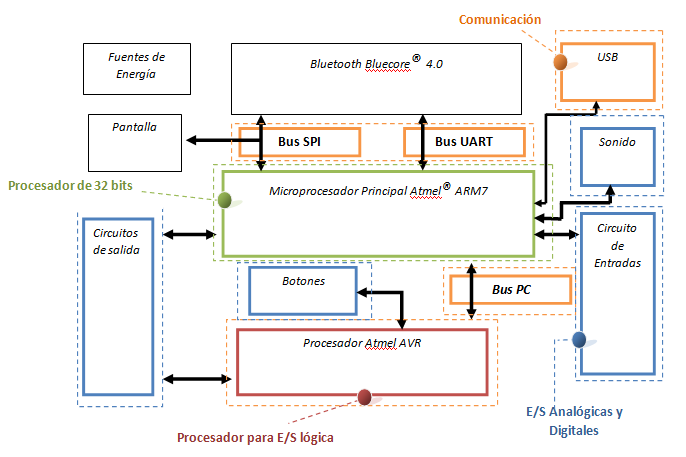
\includegraphics[width=\columnwidth]{diagramas/arquitectura-lego}
\caption{Arquitectura del SE del kit Lego NXT}
\label{fig:arquitectura-se-lego}
\end{figure}

El SE ha sido habilitado con una configuración que incluye dos servomotores conectados a las ruedas que permiten al vehículo desplazarse y con un sensor ultrasónico para la medición de la distancia hacia el obstáculo móvil.
El sensor ultrasónico funciona emitiendo ondas de sonido de alta frecuencia que son imperceptibles para el oído humano. Dichas ondas rebotan en los objetos más próximos, obteniéndose el tiempo transcurrido y calculándose así la distancia hacia los objetos.

La configuración final del vehículo es mostrada en la Figura \ref{fig:configuracion-lego}.
La descripción del proceso para armar al vehículo ha sido obtenida del manual del usuario del kit Lego NXT \cite{LEGO2014}.

\begin{figure}[!t]
\centering
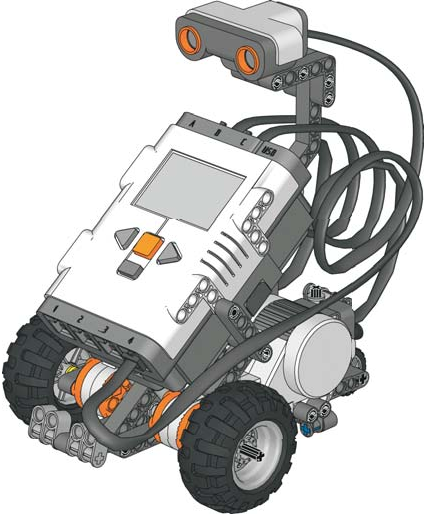
\includegraphics[width=\columnwidth]{diagramas/configuracion-lego}
\caption{Configuración del kit Lego NXT}
\label{fig:configuracion-lego}
\end{figure}

\subsection{Metodología de la implementación uno}
\label{sub:metodologia-implementacion-uno}

La idea que orilló al desarrollo de esta implementación está basada en los resultados entregados por el sensor ultrasónico para medir la distancia del SE con respecto al obstáculo móvil.
A partir de esta distancia, el robot decidiría si debía avanzar, retroceder o detenerse por completo, siempre manteniendo la distancia límite con respecto al obstáculo.

Cabe mencionar que esta implementación contempló que el sistema debería ser ejecutado durante un tiempo determinado en 10 minutos, con una potencia constante de 25\% entregada a los servomotores.
Se seleccionó el valor de 25\% con la intención de que la velocidad alcanzada por el vehículo no fuera tan alta y permitiera reaccionar adecuadamente ante los cambios en la distancia.

El pseudocódigo de esta implementación es mostrado en el Pseudocódigo \ref{alg:pseudocodigo-implementacion-uno} donde pueden identificarse las consideraciones descritas.

\begin{algorithm}
\begin{algorithmic}[1]
\STATE $p = 25$ (potencia).
\STATE $d = 0$ (distancia).
\STATE $t = 10$ (tiempo en minutos).
\STATE $d_{limite} = 40$ (distancia límite en centímetros).

\WHILE {$t>=0$}
	\STATE $d=$ leer sensor.
	\IF{$d==d_{limite}$}
		\STATE Apagar motores.
	\ENDIF

	\IF{$d>d_{limite}$}
		\STATE Avanzar con potencia $p$
	\ENDIF

	\IF{$d<d_{limite}$}
		\STATE Retroceder con potencia $p$
	\ENDIF

	\STATE $t=t-1$
\ENDWHILE
\end{algorithmic}
\caption{Implementación uno}\label{alg:pseudocodigo-implementacion-uno}
\end{algorithm}

\subsection{Metodología de la implementación dos}
\label{sub:metodologia-implementacion-dos}
La idea central de esta implementación es mantener la lectura del sensor ultrasónico de forma permanente, realizar el cálculo de la distancia entre el vehículo y el obstáculo móvil, y accionar el funcionamiento de los motores hacia adelante o hacia atrás con una potencia constante.

Tratando de anticipar los posibles errores en la precisión de la distancia entregada por el sensor ultrasónico, se definió un margen de $\pm$2cm para que el vehículo no realizara movimientos de oscilación (movimientos hacia adelante-atrás y viceversa) al encontrarse cerca de la distancia límite del obstáculo móvil.

El pseudocódigo de esta implementación es mostrado en el Pseudocódigo \ref{alg:pseudocodigo-implementacion-dos}.
Es de resaltar que cuando la distancia cae dentro del intervalo de distancia límite $\pm$2cm el envío de energía a los motores es suspendido para evitar las oscilaciones del vehículo.

\begin{algorithm}
\begin{algorithmic}[1]
\STATE $p = 50$ (potencia).
\STATE $d = 0$ (distancia en centímetros).
\STATE $d_{limite} = 40$ (distancia límite en centímetros).
\STATE $u = 2$ (umbral de error en centímetros)

\WHILE {\TRUE}
	\STATE $d=$ leer sensor.
	
	\IF{$d < (d_{limite} - u)$}
		\STATE Retroceder con potencia $p$
	\ELSIF{$d > (d_{limite} + u)$}
		\STATE Avanzar con potencia $p$
	\ELSE
		\STATE Apagar motores.
	\ENDIF

\ENDWHILE
\end{algorithmic}
\caption{Implementación dos}\label{alg:pseudocodigo-implementacion-dos}
\end{algorithm}

\subsection{Metodología de la implementación con un controlador P}
\label{sub:metodologia-implementacion-controlador-p}
En esta implementación se ha considerado la etapa de modelado del sistema, abstrayendo los detalles más importantes del entorno, obteniendo así un controlador P.

Se ha identificado que mientras que el vehículo se encuentre en movimiento la distancia hacia el obstáculo móvil describirá variaciones.
Sin embargo, la potencia utilizada para mover los servomotores no debería mantenerse constante, ya que esto introduciría oscilaciones al acercarse a la distancia límite.
Por esta razón, el comportamiento deseado involucra una adaptación de la potencia entregada a los servomotores en función de las variaciones de la distancia.

El controlador P obtenido, mostrado en la Figura \ref{fig:controlador-p-implementado}, considera los puntos descritos, haciendo uso de la magnitud del error conformado por la distancia entre el vehículo y el obstáculo móvil para adaptar de \emph{\textbf{forma proporcional}} la potencia entregada a los motores con un factor $K_p$ de 2.5. Este valor de $K_{p}$ significa que hasta los 40 cm de distancia de $d_{limite}$ la potencia entregada a los motores sería del 100\%, y será reducida a medida que la diferencia en las distancias disminuya.

\begin{figure}[!t]
\centering
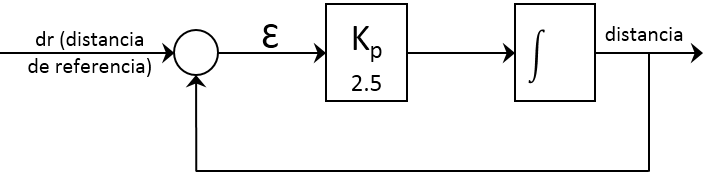
\includegraphics[width=\columnwidth]{diagramas/diagrama-controlador-p}
\caption{Controlador P implementado}
\label{fig:controlador-p-implementado}
\end{figure}

El pseudocódigo de la implementación es mostrado en el Pseudocódigo \ref{alg:pseudocodigo-implementacion-controlador-p}, de donde puede obtenerse que si el vehículo se encuentra lejos de la distancia límite, la potencia contendrá un valor alto; por el contrario, si el vehículo se encuentra cerca de la distancia límite la potencia será disminuida de forma proporcional.

\begin{algorithm}
\begin{algorithmic}[1]

	\STATE $d = 0$ (distancia).
	\STATE $d_{limite} = 40$ (distancia límite en centímetros).
	\STATE $p = 0$ (potencia).
	\STATE $K_{p} = 0$ (potencia).
	\STATE $e = 0$ (magnitud del error en centimetros).

	\WHILE {\TRUE}
		\STATE $d = $ leer sensor.
		\STATE $e = d_{limite} - d$ 
		\STATE $p = K_{p} * e$ 
		\STATE Avanzar con potencia $p$
	\ENDWHILE
\end{algorithmic}
\caption{Implementación del controlador P}\label{alg:pseudocodigo-implementacion-controlador-p}
\end{algorithm}

\section{Resultados}
\subsection{Resultados de la implementación uno} 
\label{sub:resultados-implementacion-uno}
Los resultados generados a partir por el pseudocódigo descrito en la implementación uno, demuestran que el sistema funcionó relativamente \emph{bien} puesto que en la práctica, al ejecutar el programa en el bloque NXT, reaccionaba de la forma descrita a continuación.

Si el sensor ultrasónico al momento de adquirir los valores de distancia, determinaba que el obstáculo móvil se encontraba a una distancia menor al bloque NXT, éste retrocedía.
En caso contrario, si el objeto móvil se encontraba a una distancia mayor el bloque NXT avanzaba.
Pero si el sensor determinaba que estaba a una distancia igual a la distancia límite, el bloque NXT no detenía su movimiento por completo, por lo que empezaba a generar oscilaciones.

Esta oscilación es generada debido a que los motores se encontraban funcionando con una potencia constante, por lo que al identificar que los actuadores deberían ser apagados, éstos no respondían automáticamente debido a la inercia existente en su movimiento.
Por esta razón, para el momento en el que el vehículo era detenido por completo ya había sobrepasado la distancia límite, el valor obtenido por el sensor indicaba que el vehículo tenía que desplazarse en dirección contraria, provocando la misma situación de forma indefinida.

Como ha sido mencionado, la implementación consideró un tiempo de funcionamiento determinado, por lo que al superarse este periodo de tiempo el sistema finaliza su ejecución de forma definitiva. 

\subsection{Resultados de la implementación dos} 
\label{sub:resultados-implementacion-dos}

Gracias a la introducción del umbral $\pm$ 2cm el vehículo es capaz de detenerse sin generar movimientos oscilatorios.
Sin embargo, después de realizar varias pruebas, resulta claro que la distancia entre el vehículo y la barrera móvil no es exactamente la indicada en el planteamiento del problema, lo cual es un comportamiento inadmisible en un SE crítico.

Si este umbral es eliminado, y considerando que la potencia entregada a los motores es constante, el vehículo entraría en un ciclo oscilatorio al acercarse a la distancia límite. 
Esto sucedería ya que aunque el sensor entregue la medición de la distancia a tiempo, para el momento en que el SE ordene el apagado de los motores y en que éstos se detengan por completo dicha distancia habría cambiado, repitiendo este comportamiento de forma indefinida.

Como contenido adicional, esta implementación incluyó la definición de dos tareas adicionales al control del vehículo.
Dichas tareas se enfocan a la reproducción de sonidos para denotar que el vehículo va de reversa o que se encuentra detenido.

La noción de tareas es similar a la de hilos en los sistemas operativos \emph{tradicionales}, por lo que pueden entenderse como una vía para realizar actividades de forma simultánea en el SE.
Para conseguir que las tareas llegaran a su fin, se controlaron dos variables globales a modo de tablero (memoria compartida) que al desactivarse desencadenan el término de la reproducción de los sonidos.

\subsection{Resultados de la implementación con un controlador P} 
\label{sub:implementacion_con_un_controlador_p}

La utilización del controlador P permite adaptar de forma proporcional la energía introducida al sistema en todo momento.

Por esta razón, el vehículo fue capaz de aproximarse a la distancia límite reduciendo paulatinamente la velocidad.
De esta forma los movimientos oscilatorios son eliminados, además de que se reacciona adecuadamente ante los cambios en la distancia originados al desplazar el obstáculo.
Por ejemplo, si el vehículo se encuentra a la distancia límite y el obstáculo móvil es desplazado hacia adelante, el vehículo avanza inicialmente \emph{a toda velocidad} para luego reducir paulatinamente la velocidad al acercarse al obstáculo.

Adicionalmente, la capacidad de variar la velocidad ayuda a obtener un ahorro de energía ya que los motores no se utilizan al 100\% de forma permanente.

Por lo anteriormente descrito, esta implementación ofrece una solución completa a la problemática planteada.

\section{Discusión y conclusiones}

Como fue mencionado las dos primeras implementaciones mostradas fueron desarrolladas siguiendo un proceso mental más cercano al del desarrollo de software de aplicaciones (DSA), omitiendo por completo las labores de modelado y diseño del control de SE.

Por la razón anterior, no es sorpresa que los resultados obtenidos hayan fallado en encontrar una respuesta satisfactoria en la totalidad de los casos.
No obstante, las implementaciones alcanzaron a obtener algunos detalles deseables en el funcionamiento del SE.
La Tabla \ref{tbl:aspectos-implementaciones} describe el balance de los aspectos tanto positivos como negativos de las implementaciones, permitiendo obtener un balance conciso de las mejoras que pueden ser aplicadas en estos enfoques.

\begin{table*}[!t]

\renewcommand{\arraystretch}{1.3}
\caption{Aspectos positivos y negativos de las implementaciones realizadas}
\label{tbl:aspectos-implementaciones}
\centering
\rowcolors{5}{gray!0}{gray!15}
\begin{tabular}{p{4cm}p{4cm}p{4cm}p{4cm}}
\toprule

\multicolumn{2}{c}{Implementación 1} & \multicolumn{2}{c}{Implementación 2}\\
\cmidrule(r){1-2}  \cmidrule(r){3-4}

\multicolumn{1}{c}{Positivo} & \multicolumn{1}{c}{Negativo} & \multicolumn{1}{c}{Positivo} & \multicolumn{1}{c}{Negativo} \\
\midrule

% + implementación 1
El vehículo avanzó cuando el obstáculo móvil se alejaba.
&
% - implementación 1
El vehículo realizó oscilaciones cuando el obstáculo móvil se encontraba cercano a la distancia límite.
&
El vehículo avanzó cuando el obstáculo móvil se alejaba.
% + implementación 2
&
% - implementación 2
Se introdujo un margen de error que es inadmisible en un SE de labor crítica.
\\

% + implementación 1
El vehículo retrocedió cuando el obstáculo móvil se acercaba
&
% - implementación 1
Se consideró que el tiempo de ejecución del software era finito.
&
El vehículo retrocedió cuando el obstáculo móvil se acercaba
% + implementación 2
&
% - implementación 2
La potencia entregada a los motores es constante, no es modificada al estar cerca de la distancia límite.
\\

% + implementación 1
% Nada
&
% - implementación 1
No se consideró que el sensor ultrasónico pudiera contar con un margen de error o retrasos al obtener la distancia.
&
% + implementación 2
Se consideró que las lecturas entregadas por el sensor pueden contener errores.
&
% - implementación 2
% Nada
El flujo del programa considera un caso en el que \emph{no se hace nada}.
Esto significa que el SE no está reaccionando activamente ante todas las entradas.
\\

% + implementación 1
% Nada
&
% - implementación 1
Se consideró que el apagado de los motores se traduciría instantáneamente en la detención del vehículo; por ello no se implementó una reducción paulatina de la velocidad.
&
% + implementación 2
Se consideró que el sistema debe funcionar de forma permanente.
&
% - implementación 2
\\
\bottomrule
\end{tabular}
\end{table*}

A manera de conclusión, vale la pena mencionar que es crucial realizar la abstracción de los detalles más relevantes del mundo real para obtener el modelo a utilizar por el SE. 
Puede tomarse como ejemplo la problemática mostrada en este reporte y cómo los enfoques carentes del modelo y controlador no pudieron dar una solución completa al problema.

Además, es importante mencionar que a pesar de que un enfoque basado en la perspectiva del DSA podría alcanzar a dar respuesta a las necesidades de un SE, tiende a alejarse de la naturaleza del problema, omite aspectos elementales de diseño y obtiene un producto lógico más complejo que el equivalente desde la perspectiva de control.

En este sentido, se ha identificado que una diferencia importante en ambas disciplinas se encuentra precisamente en la parte del análisis y diseño de los requisitos.
A pesar de que ambas consideran el diseño, la perspectiva del DSA se centra por completo en atender requisitos de un cliente, mientras que la perspectiva de control de SE considera elementos físicos inherentes a la naturaleza del problema, aspectos pocas veces abordados en el DSA.

\bibliographystyle{plain}
\bibliography{bibliography/references}
\end{document}